
% --------------------------------------------------------------
\begin{chapter}{Surrogate Assisted Decision Making \label{Chap:optimisation}}

The solution to a Bayesian decision problem is
\begin{equation}
  \bx^{*} = \argmax_{\bx \in \mathcal{X}} U(\bx)
\end{equation}
where $\bx$ is a decision from $\mathcal{X}$, the set of all feasible decisions and $U(\bx) = \E \{ u(\bx) \}$ is the expected utility of a decision where $u(\cdot)$ is the utility function. When making decisions under certainty, $u(\bx) = \E \{ u(\bx) \} $. Here, expectation is taken with respect to the decision maker's (DM's) beliefs over (unknown) parameters $\bm{\theta}$. This could be prior beliefs $\pi(\bm{\theta})$ or they could in fact be posterior beliefs $\pi(\bm{\theta} | \by)$ when relevant data $\by$ is available.

Hence, once the decision problem has been defined by an appropriate set of beliefs, the decision problem is reduced to an optimisation problem. Even though we have reduced the problem, optimisation is frequently a non-trivial task. The difficulty of the problem is increased when the utility function is expensive to compute. This can be because $u(\bx)$ itself is expensive to compute or depends on the output of one or more computationally expensive simulators \citep{Williamson2012}. The latter situation is commonly seen in Bayesian Design of Experiments when viewing the posterior as the output of a computationally expensive simulation (such an MCMC scheme) \citep{Ryan2016}.

We now discuss the various types of optimisation problems that arise and the ways in which to solve them.


\section{Discrete Problems}
\subsection{Small, Discrete Problems}
Suppose that there is no obvious structure to be exploited in the decision problem or the number of decisions that can be taken is small. For instance, \citet{Oakley2009} considers taking one of three medical treatments, that is $\mathcal{X} = \{ \bx_1, \bx_2, \bx_3\}$. Although we can express beliefs about the outcomes in a numerical way (e.g. probability of recovery), there isn't a nice structure in the decision space that can be leveraged. For example, $\bx_1 = \text{Antibiotics}$ and $\bx_2 = \text{Surgery}$ provides little structure. There is little we can do other than evaluate $U(\bx_i)$ and see which gives us the largest expected utility.

When the decision is made under uncertainty, the simplest way forward us to use a Monte Carlo approximation of $U(\bx_i)$. If evaluating $u(\cdot)$ is expensive because, for example, the utility of a decision depends on the result of a complex computer model we may wish to construct an emulator for $u(\cdot)$ as a function of uncertain quantities $\bm{\theta}$. That is, construct a surrogate $\hat{u}(\theta)$ and propagate probabilistic beliefs $\pi(\bm{\theta})$ through $\hat{u}(\bm{\theta} \mid \bx_i)$. This is precisely what \citet{Oakley2009} does, and achieves a tractable approximation to $U(\bx_i)$ using a GP emulator as a fast surrogate for $u(\bm{\theta \mid \bx_i})$.

\subsection{Structured, Discrete Problems}

Some decision problems are discrete in nature but perhaps far too complex for a brute force computation and it might not be possible to construct a surrogate. In some situations we cannot solve the decision problem exactly because of these computational constraints. We must settle for a `good' solution in the time available.

In complex, discrete problems the expected utility surface can be very rough with respect to the decision space. A famous example of such a problem is the Travelling Salesman Problem (TSP) in which a salesman aims to visit a fixed set of locations which minimise an outcome such as time taken or distance covered. Phrasing as a decision problem, if $\ell(\bx)$ is the distance of the path taken by the salesman we would take $U(\bx) \propto \ell(\bx)$. In this case, a small tweak in the path might lead to a not so small change in $U(\bx)$ \citep{Gutin2007}.

A really simple approach to the problem is random search. Take a random sample $\mathcal{X}_0 = \{ \bx_1, \bx_2, \ldots, \bx_n\}$ from $\mathcal{X}$. Then an approximation to the optimal decision is $\hat{\bx} = \argmax_{\bx \in X_0} U(\bx)$. If the computational budget is large enough, we would find $\bx^{*}$, but that's often a big ``if'' in practice - convergence can be incredibly slow. Beyond this, random search serves as a benchmark: if random search does better than a seemingly more intelligent method, then perhaps the method isn't so intelligent or is ill-suited to the problem.

An adaptation of random search is stochastic optimisation. A common example is simulated annealing (SA) which is inspired by the process of annealing in metallurgy \citep{Schneider2006}. SA is one of many stochastic optimisers but does quite well when the decision surface is very rough. Given a candidate solution $\bx'$ and a `current' solution $\bx_t$ we take $\bx_{t+1} = X_{t+1}$ where $X_{t+1}$ is a random variable which takes the value $\bx'$ with probability $\alpha( \bx' \mid \bx_{t}, t)$ and $\bx_t$ otherwise. The candidate decision will typically be a modified version of $\bx_t$. If the decision space is the real line, we might form $\bx'$ by $\bx' = \bx_t + N(0, \sigma^2)$.  Typically $\alpha(\bx' \mid \bx_{t}, t)$ is close to $1$ at the start of the routine and slowly converges to $0$ (or a very small value) as $t$ gets large. Also, $\alpha(\bx' \mid \bx_{t}, t)$ should be biased towards the decision with largest $U$ as $t$ gets large. A common form for alpha is
\begin{equation}
  \alpha(\bx' \mid \bx_{t}, t) = \min \left\{  \exp\left[-\frac{U(\bx_t) - U(\bx')}{Kt}\right], 1\right\}
\end{equation}
where $K$ is a tuning parameter which controls the rate of the annealing schedule. SA can be thought of as the optimisation equivalent of Markov Chain Monte Carlo (MCMC). In MCMC we propose a new value $\theta^{*}$ for a parameter value $\theta$ and accept $\theta^{*}$ as a draw from $\pi(\theta |\bx)$ with an acceptance probability $\beta(\theta, \theta^{*})$, where $\beta(\cdot, \cdot)$ is the Metropolis-Hastings ratio. SA is similar, but SA aims to `climb up' the landscape, whereas MCMC aims to explore the landscape.


Other discrete structures that can be exploited are permutations; consider a set of tasks $\{T_1, T_2, \ldots, T_J\}$. If there are $J$ tasks to complete, there are at most $J!$ permutations which need to be considered. For moderately small $J$, $J!$ can be very large and grows incredibly quickly ($3! = 6$, $6! = 720$, $10! = 3628800$ ). Computing $U(\bx)$ all possible $\bx$ can quickly become very time consuming, especially if $U(\cdot)$ is expensive for just one $\bx$. To alleviate this, \citet{Wilson2018} use a surrogate inspired by the Benter model \citep{Benter1994}.

\section{Continuous Problems}

If the decision problem is continuous, e.g. $d \in \mathcal{D} \subset \mathbb{R}$ and we have relatively easy access to $U(d)$ we can use standard optimisation routines like \verb|optim| in \verb|R| or even calculus methods.  By `easy access' we mean that $U(d)$ is available in closed form or we have access to highly accurate approximations (e.g. Monte Carlo approximations from a very large sample).

However, evaluation of $U$ might be sufficiently difficult to make standard optimisation methods cumbersome. If evaluations of $U$ or $u$ are limited for computational or financial reasons (e.g. running simulations on a web server, include collection of real data or human interaction) we would want to use a surrogate to speed up the optimisation.

Broadly, we can use a surrogate to perform optimisation in two ways. The simplest way is to construct a surrogate $\hat{U}(\bx)$ and maximise the surrogate to (approximately) solve the decision problem. For examples of this approach see \citep{Wilson2018, Overstall2017}.

\section{Bayesian Optimisation}

An alternative approach is construct a surrogate $\hat{U}(\bx)$ and rather than maximise $\hat{U}(\bx)$ we use the surrogate to tell us where to next run the expensive function according to some rule. This often goes by the name \textit{Bayesian Optimisation} (BayesOpt). The core idea behind BayesOpt is to construct an emulator for $U(\bx)$ and use this to guide our search towards $\bx^{*}$. Although a lot of the BayesOpt language is plagued by machine learning jargon, BayesOpt is really just sequential design. BayesOpt has found itself to be useful in a variety of optimisation problems where the surface to be optimised may possess multiple local optima, derivatives are not available/difficult to approximate and the function is thought to be quite smooth \citep{Frazier2018}. A common application is tuning machine learning algorithms \citep{Joy2016, Snoek2012}. BayesOpt dates back to at least \citet{Mockus1975} who used (Bayesian) linear models but its current form (GP modelling) has stemmed from \citet{Jones1998}. BayesOpt can be viewed as a sequential design strategy for global maximisation (or minimisation) expensive black-box functions, see \citet{Frazier2018} for a review. The

To perform BayesOpt we typically specify a GP prior over the unknown function, $f(\cdot)$, which is possibly obfuscated by noise and usually induced by a computer simulator. We will make a slight diversion here and think about general purpose functions $f(\cdot)$ rather than utility functions. Suppose we observe $y(\bx) = f(\bx) + \varepsilon(\bx)$ where $f(\cdot)$ is the function to be maximised and $\varepsilon(\bx)$ is (possibly input dependent) noise which is usually assumed to be Gaussian. We start by specifying the joint model for $(\by^T, f(\bx)^T)$ and use the conditional Normal equations to provide the posterior moments for $f(\bx) \mid \by$


\begin{align}
  \begin{pmatrix} \by \\ f(\bx) \end{pmatrix}
    &\sim \mathcal{N} \left\{
    \begin{pmatrix} \mu(X) \\ \mu(\bx) \end{pmatrix}, \begin{pmatrix} \Sigma_{X, X} & \Sigma_{X, \bx} \\ \Sigma_{\bx, X} & \sigma^2 \end{pmatrix}
    \right\} \\
    f(\bx) \mid \by &\sim \mathcal{N}(\mu_{*}(\bx), \sigma^2_* ) \\
    \mu_*(\bx) & = \mu(\bx) + \Sigma_{\bx, X}(\Sigma_{X, X}+\lambda^2(X)I)^{-1}(\by - \mu(X))\\
    \sigma^2_* &= \sigma^2 - \Sigma_{\bx, X}(\Sigma_{X, X}+\lambda^2(X)I)^{-1}\Sigma_{X, \bx}
\end{align}

where $X$ is the locations at which the simulator has been run, $\mu(\cdot)$ is the prior mean, $\Sigma_{X, X} = \var(\by$, $\Sigma_{\bx, \bx} = \var\{f(\bx)\}$, $\Sigma_{X, \bx} = \Sigma_{\bx, X}^T = \cov(y(X), f(\bx))$ and $\lambda^2(X)I = \var(\varepsilon(X))$.

\subsection{Acquisition Functions}

Once the emulator has been fit to the data, we then need to figure out where to next run the computer model. This is done by an \textit{acquisition function}. The acquisition function is a function of the posterior distribution on $f(\cdot)$. We now introduce slightly different notation for the posterior on $f(\cdot)$. Suppose we have observed $n$ runs of the simulator $\mathcal{D}_n = \{(x_1, y_1), (x_2, y_2), \ldots, (x_n, y_n)\}$. The `time $n$' posterior for the unknown function (after observing $n$ runs) is denoted $\pi_n(f(\cdot) \mid \mathcal{D}_n, \Theta_n)$ where $\Theta_n$ are the time $n$ GP hyperparameters. We will abuse notation here and use $\pi_n(f(\cdot))$ as shorthand for $\pi_n(f(\cdot) \mid \mathcal{D}_n, \Theta_n)$.  If $g(\cdot)$ is some function of $f(\bx)$ then denote $\E\{g(f(\bx)) \mid \mathcal{D}_n, \Theta \}$ by $\E_n \{ g(f(\bx)) \}$.

We introduced this notation because many acquisition functions can be expressed as expectations. This means that many acquisition functions have a decision theoretic justification as Bayes optimal decisions. We define the current `best' solution to be
\begin{equation}
  \hat{\bx}_n = \argmax_{x \in X_n} \E_n \{ f(\bx) \}
\end{equation}
where $X_n$ is the set of points at which the simulator has been run. Let $y^{*}_n = \E_n \{ f(\hat{\bx}_n) \}$ and for an arbitrary $\bx$ let $\mu_n(\bx) = \E_n \{ f(\bx) \}$ and $\sigma^2_n = \var_n\{ f(\bx) \} = \E_n \left\{  \left[ \E_n(f(\bx)) - f(\bx)\right]^2  \right\} $.
\subsubsection{Probability of Improvement}

The simplest acquisition function is perhaps the probability of improvement (PI) denoted $\alpha_{PI}$. Suppose we have the following utility function over $f(\bx)$:

\begin{equation}
  \tilde{\alpha}_{PI}(\bx) =
  \begin{cases}
    1,& f(\bx) > y^{*}_n \\
    0,& f(\bx) \leq y^{*}_n
  \end{cases}
\end{equation}
that is, an indicator utility function returning $1$ when we improve our best value and returning $0$ when we don't improve the best value. This expresses the belief that all improvements, regardless of magnitude, are equally preferable. We then have $\alpha_{PI}(\bx)  = \E_n \{ \tilde{\alpha}_{PI}(\bx) \}$. The expectation of an indicator function is just the probability of the event in question, thus we have
\begin{align}
  \alpha_{PI}(\bx) &= \p(f(\bx) > y^{*}_n)\label{Eq:prob-imp}\\
   &= \Phi\left(\frac{ \mu_{n}(\bx)  - y^{*}_n }{\sigma_{n}(\bx)}\right). \label{Eq:prob-imp-gp}
\end{align}
Now, no matter what the statistical model, \Cref{Eq:prob-imp} is the probability of improvement. Under GP assumptions, the probability of improvement can be expressed as \Cref{Eq:prob-imp-gp}.

\subsubsection{Expected Improvement}

A fairly obvious criticism of PI as an acquisition function is that is treats all improvements equally, regardless of the magnitude of the improvement. Suppose that $y^{*}_n = 0$ and consider two values of $\bx$ denoted $\bx_1$ and $\bx_2$. Suppose $f(\bx_1)  \sim N(0, 1)$ and $f(\bx_2) \sim N(0, 10)$. Both of these candidate values have the same probability of improvement (namely, $0.5$) but the potential gains under $\bx_2$ are much larger than the potential gains under $\bx_1$.

This motivates \textit{Expected Improvement} which gives a reward proportional to the improvement. First we define the improvement by
\begin{equation}
  \tilde{\alpha}_{EI}(\bx) = \max\{0, f(\bx)-y^{*}_n\}.
\end{equation}
This is intuitive: if $f(\bx) \leq y^{*}_n$ our best value hasn't improved (but has helped us learn about $f(\cdot)$ so is not wasteful). But if $f(\bx) > y^{*}_n$ then we have improved our current largest value of $f(\cdot)$ by $f(\bx) - y^{*}_n$. The expected improvement is then the expected value of the improvement, where expectation is taken with respect to $\pi_n(f(\bx))$:
\begin{equation}
  \alpha_{EI}(\bx)  = \E_n \{  \tilde{\alpha}_{EI}(\bx) \}.
\end{equation}
Under standard GP assumptions, we have an analytic expression for EI in terms of the Normal CDF and PDF.  Here we aim to maximise $f(\cdot)$ so the acquisition function can be expressed as

\begin{equation}
  \alpha_{EI}(\bx) = \begin{cases}
                      \sigma_n(\bx)\Phi\left(\frac{\mu_n(\bx)-y^{*}_n}{\sigma_n(\bx)}\right) + (\mu_n(\bx) - y_n^{*})\phi\left(\frac{\mu_n(\bx)-y^{*}_n}{\sigma_n(\bx)}\right)&  ,  \sigma_n(\bx) > 0 \\
                      0 & ,  \sigma_n(\bx) = 0
                      \end{cases}
\end{equation}
the EI is $0$ when $\sigma_n(\bx) = 0$ because when $\sigma_n(\bx) = 0$ we know the value of $f(\bx)$ precisely. $f(\bx)$ will either be $y_n^{*}$ or smaller than $y_n^{*}$ and hence offers no improvement. Although EI was constructed with deterministic problems in mind, it generalises easily to the stochastic case.

There are many extensions to EI which take into account problem structure. Examples include optimisation under unknown (black-box) constraints which aims to learn the optimum input/output and the constraints \citep{Gramacy2010} and taking advantage of parallel computing with batch/multi-point EI \citep{Marmin2015}.

\subsubsection{Upper Confidence Bound}

Another common acquisition function is the Upper Confidence Bound (UCB) approach \citep{Srinivas2009}.
The UCB acquisition function is, under a GP model for $f(\cdot)$,

\begin{equation}
  \alpha_{UCB}(\bx \mid \nu_n) = \mu_n(\bx) + \nu_n \sigma_n(\bx).
\end{equation}
UCB was proposed with maximisation in mind but if minimisation is required we can use the lower confidence bound instead.
\begin{equation}
  \alpha_{LCB}(\bx \mid \beta_n) = \mu_n(\bx) - \nu_n \sigma_n(\bx).
\end{equation}

where $\nu_n > 0$ are a sequence of tuning parameters controlling the exploration-exploitation trade-off. If desired, we can take $\nu_n = \nu$ for all $n$. Here the trade-off is explicit; letting $\nu_n = 0$ leads to a pure exploitation regime: maximise the posterior mean. Letting $\nu_n \to \infty$ leads to picking the point with highest uncertainty which is essentially exploration. Choosing a moderate value of $\nu_n$ leads to a trade-off. The UCB acquisition function is sometimes called an `optimistic' approach; we are choosing $\bx_{n+1}$ based on an upper estimate for $f(\bx_{n+1})$.

Although not immediately obvious, we can actually write this function as the expected value of a random variable \citep{JamesWilson2018}. Note that
\begin{equation}
 \alpha_{UCB}(\bx \mid \nu_n) = \int_{\mu(\bx)}^{\infty} \tilde{y} \phi\left\{ \frac{\tilde{y} - \mu(\bx)}{\tilde{\sigma}(\bx)} \right\} \diff \tilde{y}
\end{equation}
hence we have
\begin{equation}
   \alpha_{UCB}(\bx \mid \nu_n) =\E_{\tilde{y}} \{\tilde{y} \times \mathbb{I}(\tilde{y} > \mu(\bx))\}
\end{equation}
where $\tilde{y} \sim \mathcal{N}(\mu(\bx), \tilde{\sigma}^2(\bx))$ and $\tilde{\sigma}(\bx) = \frac{1}{2}\pi \nu_n^2 \sigma^2(\bx)$. Therefore $\alpha_{UCB}(\bx)$ can be interpreted, in a decision theoretic context, as the expected value of a linearly transformed and truncated version of $f(\bx)$.
\subsubsection{Thompson Sampling}

There is also a stochastic approach to BayesOpt; Thompson Sampling (TS). TS originated in two-armed bandit problems \citep{Thompson1933} and has enjoyed recent praise in multi-armed bandit problems as a simple and effective heuristic \citep{Scott2010, Chapelle2011}. The idea behind TS is to draw a random function $g(\cdot) \sim \pi_n(f(\cdot))$ and then the next point at which to run the simulator is
\begin{equation}
  \bx_{n+1} = \argmax_{\bx \in X} g(\bx).
\end{equation}

In words, the acquisition function is the maximiser of a realisation of $f(\cdot)$. A drawback of TS is that we can't actually draw a random function from $\pi_n(f(\cdot) )$. The best we can do is first choose a set of points $\tilde{X}$ at which we would like to estimate $f(\cdot)$ and then draw the values $\bm{g} = g(\tilde{X})$ from a multivariate Normal distribution. This can cause problems in high dimensional settings due to the curse of dimensionality. We can also `extend' this realisation, whilst preserving the realisations we already have, by adding rows to the lower Cholesky decomposition of $\var \{ f(X) \}$. This means we can't exactly maximise $g(\cdot)$ when the decision space is either continuous or large and discrete. However, the three earlier acquisition functions all need to be maximised via some inner optimisation routine like \verb|optim|. The TS acquisition is trivially maximised via a lookup table.

All the discussed acquisition functions are plotted in \Cref{Fig:acq-fns}. They all correspond to the function and corresponding emulator in \Cref{Fig:example-fn}. In this particular example, PI, EI and UCB are all maximised in roughly the same place, two of the TS samples are also maximised in the same place whereas one TS sample (green) is maximised at just over $x= 0.8$. Remember that this is telling us where to next run the simulator rather than a prediction of where the maximum actually is.

\begin{figure}[h]
  \centering
  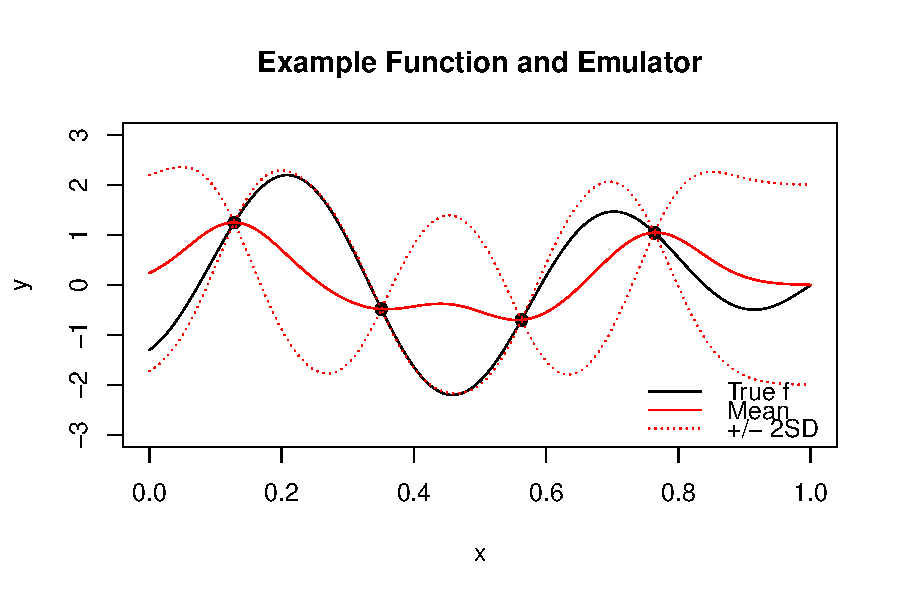
\includegraphics[width=\textwidth]{fig-optim/example-fn.pdf}
  \caption{An example function to be optimised via BayesOpt with a corresponding emulator.}
  \label{Fig:example-fn}
\end{figure}
\begin{figure}[h]
  \centering
  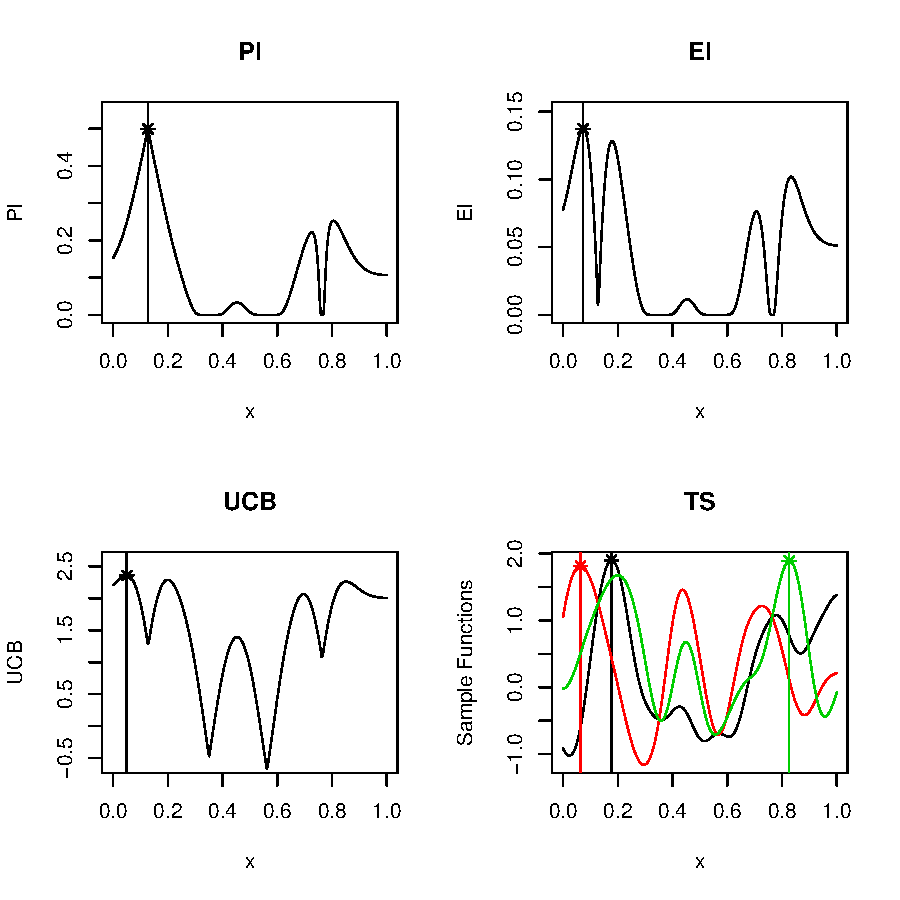
\includegraphics[width=0.8\textwidth]{fig-optim/classic-acquisition.pdf}
  \caption{Plots of acquisition functions for the function and emulator in \Cref{Fig:example-fn}. Vertical lines correspond to the maximiser of the acquisition function with the asterisk being the the coordinates of the maximum. Three possible acquisition functions for TS are shown.}
  \label{Fig:acq-fns}
\end{figure}
\subsection{Online GP Prediction}
 BayesOpt is, by design, a sequential procedure. Thus we add data to the model online or as it arrives. GP prediction depends on the inversion of a matrix of size $n \times n$. This is well known to be slow (usually $\mathcal{O}(n^3)$) and numerically unstable.

 It turns out that, under a simple partition of $\Sigma_{n+1}$, that the time $n+1$ precision matrix $\Omega_{n+1}$ can be expressed efficiently in terms of $\Omega_n$ and the partitioned $\Sigma_{n+1}$.

 Consider the following partition of $\Sigma_{n+1}$ with a diagonal nugget term added:
 \begin{equation}
  \Sigma_{n+1} + \lambda^2(X_{n+1}) = \begin{pmatrix}
                  \Sigma_n + \lambda^2(X_n)I_n & c(\bx_{n+1}, X_n) \\
                  c(\bx_{n+1}, X_n)^T  & \sigma^2 + \lambda^2(\bx_{n+1})
                  \end{pmatrix}
 \end{equation}
 where $c(\bx_{n+1}, X_n)$ is the column vector of covariances between $\bx_{n+1}$ and the rows of $X_n$. Note that $\Sigma_n + \lambda^2(X_n)I_n = \Omega_n ^{-1}$.
We then have

\begin{equation}
  \Omega_{n+1} = \begin{pmatrix}
                  \Omega_n + k k^T /s & -k/s \\
                  -k^T/s & 1/s
                 \end{pmatrix}
\end{equation}
where $k = \Omega_n c(\bx_{n+1}, X_n)$ and $s = \sigma^2 + \lambda^2(x_{n+1}) -  c(\bx_{n+1}, X_n)^T k$. A proof of this result is straightforward by simply performing the calculation $\Omega_{n+1} (\Sigma_{n+1} + \lambda^2(X_{n+1})$; see \citet{Gentle2007} Section $3.4$ for the result and Exercise of Section $3$ for sketch proof. This works only if we condition on GP hyperparameters (e.g. do hyperparameter inference offline, or in batches). The only new information we need is $c(\bx_{n+1}, X)$ and $\lambda^2(\bx_{n+1})$. This amount to calculating a length $n$ vector of covariances. If we choose a constant nugget effect, $\lambda^2(\bx_{n+1})$ is already known.

\section{The Inner Optimisation Problem}

BayesOpt rephrases the problem of maximising $f(\bx)$ to training a GP model, updating precision matrices and maximising an acquisition function, $\alpha(\bx)$. Since $\alpha(\bx)$ is much cheaper to evaluate than $f(\bx)$, maximisation of $\alpha(\bx)$ is feasible (but is not always easy!). For instance, although \Cref{Fig:example-fn} shows a fairly basic, $1$ dimensional emulator, the corresponding acquisition functions (\Cref{Fig:acq-fns}) are quite nasty. They are highly multimodal and in many cases will be high dimensional. However, to maximise $\alpha(\bx)$ we can use anything from the standard optimisation literature.

The simplest thing to do is a large grid/random search. Since $\alpha(\bx)$ should be relatively cheap to compute, in many cases this will give us a `good' solution.

However, we can often do better than this by using standard optimisation routines such as BFGS/L-BFGS-B. These optimisation methods require $\frac{\partial \alpha(\bx)}{\partial \bx}$. This can be found by finite differencing but can also be found exactly in many cases (or doing some mathematics leads to a sensible approximation). Since acquisition functions are functions of $\mu_n(\bx)$ and $\sigma^2_n(\bx)$ we will first need to derive the gradient of these quantities. The gradient of many acquisition functions will follow from standard differentiation rules. In this section we will assume a constant prior mean $\beta$ and a constant nugget effect $\lambda$. Let $K_n = \Sigma_n + \lambda^2 I_n$ be the data covariance matrix. Much of the remainder of this chapter depends on matrix and vector calculus, see \citet{Wand2002} and \citet{Deisenroth2020} (Chapter $5$) for details.


\subsection{Gradient of the Covariance Function}

The posterior moments from a GP depend explicitly on the vector of covariances between the function at the (untried) input, $\bx$, and the inputs at which the model has been run, $X_n$. The gradient of the covariance will depend on the exact form of the covariance function, here we consider the squared exponential covariance function.
Here, we consider the parameterisation
First we find the gradient of the covariance between $\bx$ and a single input $\bx_i$. We paramterise the covariance function such that the lengthscales are stored in a (diagonal) matrix $D$ and thus the squared distance between $\bx$ and $\bx_i$ is $(\bx - \bx_i)^T D^{-1} (\bx - \bx_i)$. Assume that the length of $\bx$ is $p$.
\begin{align}
  \dbx	c(\bx, \bx_i) &= \dbx \sigma^2 \exp\{ -(\bx - \bx_i)^T D^{-1} (\bx - \bx_i) \}\\\nonumber
  &=\sigma^2 \dbx \{ -(\bx - \bx_i)^T D^{-1} (\bx - \bx_i) \} \exp\{ -(\bx - \bx_i)^T D^{-1} (\bx - \bx_i) \}\\\nonumber
  &= -2 D^{-1} (\bx - \bx_i) c(\bx, \bx_i)
\end{align}
 which is a length $p$ vector.


 Now differentiation of $c(\bx, X)$ results in a Jacobian term:
 \begin{align}
 	\dbx c(\bx, X) &= \begin{pmatrix}
 		\frac{\partial c(\bx, \bx_1)}{\partial x_1} & \frac{\partial c(\bx, \bx_2)}{\partial x_1} & \ldots & \frac{\partial c(\bx, \bx_n)}{\partial x_1} \\
    \frac{\partial c(\bx, \bx_1)}{\partial x_2} & \frac{\partial c(\bx, \bx_2)}{\partial x_2} & \ldots & \frac{\partial c(\bx, \bx_n)}{\partial x_2} \\
 		\vdots & \vdots & \ddots & \vdots\\
 		\frac{\partial c(\bx, \bx_n)}{\partial x_p} & \frac{\partial c(\bx, \bx_2)}{\partial x_p} & \ldots & \frac{\partial c(\bx, \bx_n)}{\partial x_p} \\
 \end{pmatrix}\nonumber\\
 &=-2D^{-1}\begin{pmatrix}
 	(\bx - \bx_1)^T c(\bx, \bx_1)\\
 	(\bx - \bx_2)^T c(\bx, \bx_2)\\
 	\vdots\\
 	(\bx - \bx_n)^T c(\bx, \bx_n)\\
 \end{pmatrix}^T\nonumber\\
   &=-2D^{-1} \tilde{X}^T \diag \{ c(\bx, X) \}
 \end{align}
which is a $p \times n$ matrix. Here we introduced $\tilde{X} = (\bx- \bx_1, \bx-\bx_2, \ldots, \bx-\bx_n)^T$. Note that the $c(\bx, \bx_i)$ terms are just scalars so we can factorise into the above form.

\subsection{Gradient of $\mu_n$}

Now the gradient of $\mu_n(\bx)$ follows in a fairly straightforward way because $\mu(\bx)$ is a linear transformation of $c(\bx, X)$.

\begin{align}
	\dbx \mu_n(\bx) &= \dbx \left\{  \beta + c(\bx, X)K^{-1}(\by - \beta) \right\}\nonumber \\
	& = 0 + \dbx \{ c(\bx, X) \} \bm{e} \nonumber\\
	&= -2D^{-1} \tilde{X}^T \diag \{ c(\bx, X) \}
	\bm{e}
\end{align}
where $\bm{e}=K_n^{-1}(\by - \beta)$.

\subsection{Gradient of $\sigma_n^2$}

Recall $\sigma_n(\bx) = \sigma^2 - c(\bx, X)K_n^{-1}c(\bx, X)^T$. The gradient of $\sigma^2(\bx)$ follows in a similar way to $\mu_n(\bx)$ but with the addition of the chain rule. Let $\bm{w} = c(\bx, X)$.
\begin{align}
  \dbx \sigma^2(\bx) &= \dbx \{ \sigma^2 - c(\bx, X)K_n^{-1}c(\bx, X)^T \} \nonumber\\
  &=-\dbx \{ c(\bx, X)K_n^{-1}c(\bx, X)^T \} \nonumber\\
  &=- \dbx{c(\bx,X)} \frac{\partial}{\partial \bm{w}}\{ \bm{w} K^{-1} \bm{w} \} \nonumber\\
  &= -4D^{-1} \tilde{X}^T \diag( c(\bx, X))K^{-1}c(X, \bx).
\end{align}

Now since $\alpha(\bx)$ is a scalar, the gradient of $\alpha(\bx)$ is often straightforward given $\dbx \mu_n(\bx)$ and $\dbx \sigma^2_n (\bx)$. The gradient of $\alpha(\bx)$ will depend on its exact form so will have to be derived on a case-by-case basis.

\section{Decision Support for Athena}

A major concern for a wind farm operator is the logistic aspects of repairing turbines. A wind farm operator may have to wait for a window of fair weather to perform a repair, this is also subject to an appropriate repair boat being available. Ultimately, repair relies on there being a spare component available to replace the broken one. Recent modifications to the model allow a decision maker to investigate the impact of limited spare components on availability. Athena represents a wind turbine as being constructed of $9$ key subassemblies: gearbox, generator, frequency converter, transformer, main shaft bearing, the blades, tower, foundations and the catch all. Each type of subassembly degrades according to Weibull hazard functions until it eventually fails and is in need of repair. More serious damage to a subassembly will require the component to be replaced. This requires specialist components which may be in limited supply at a warehouse close to the dock. Carefully choosing the total number of spare components and how to distribute the space is very important. Spare components are highly specialised and if we were to simply order in a new component upon the discovery of a failure we may be waiting, in extreme cases, many months for the repair to take place \citep{Ferdinand2018}. It therefore makes sense to order more spare parts when the number of spare parts of type $j$ goes below some threshold. We choose the threshold to be $p_js_j$ where $s_j$ is the maximum number of spare parts of type $j$ and $p_j \in (0,1)$ is a proportion. The combinations of $(p_1, \ldots, p_9)$ is the `restoration policy'.

We propose a decision theoretic solution to the problem. In particular, we advocate the use of a subjective Bayesian approach in which the utility function is elicited from the decision maker (DM). `Off the shelf' utility functions have found themselves to be popular in well-defined scenarios such as Bayesian experimental design \citep{Ryan2016}. A subjective utility function allows the decision maker to fully embrace the uniqueness of the problem. In planning a wind farm the DM must consider the local geography and resources, for example.  The elicitation of utility is usually done by comparing a certain consequence $c$ to a lottery $ L =  [c_1, c_2 ; 1-p]$ which returns consequence $c_1$ with probability $1-p$ and consequence $c_2$ with probability $p$. We take the worst consequence to have $u(c_1) = 0$ and the best consequence satisfies $u(c_2) = 1$. Now, if $c$ is equally preferable to $L$ then $u(c) = p \in [0,1]$ \citep{Smith2010}. Keeping utilities on the $[0,1]$ scale means the utility function is interpretable in terms of lotteries and probabilities but also allows the construction of multi-attribute utility functions -- utility functions which take into account competing objectives -- to be much more straightforward \citep{Gonzalez2018, Morton2018}. The combination of best warehouse allocation of spare parts and spare part restoration policy will be the choice which maximises the DM's expected utility function. A crucial attribute to the decision problem is the availability time series output by Athena. The time series is stochastic; all decisions are made under uncertainty. Another issue that models, and utility functions, are imperfect representations of reality.
%Athena has a large number of inputs, many are that of probability distributions which relate to component lifetimes. These parameters of these probaility distributions were elicited from experts. There are many resources which are limited in offshore wind, some of these are expressed as parameters in the Athena model. For instance, specialist boats may need to be hired to move spare components from land to a turbine in need of repair.


%  We focus on spare parts needed for $9$ key turbine subassemblies. Spare parts need to be stored in a warehouse of finite size. It is most important to a decision maker to get the choice of warehouse correct, but there are other decisions to be made along side this which we should also account for. We are interested in choosing the numbers of spare components to store in the warehouse. There are $9$ subassemblies so we have $9$ types of spare component. Different components fail at different rates (according to the expert elicted quanitites) so choosing the numbers of spares, subject to filling the warehouse is also an important decision to be made.

Since Athena is both computationally expensive and stochastic an efficient approach to maximising expected utility is Bayesian optimisation (BayesOpt). The most common approach in BayesOpt is to model the expensive function, $f(\bx)$ as a Gaussian process (GP). We might not directly observe $f(\bx)$ but some noisy version $y(\bx) = f(\bx) + \varepsilon(\bx)$. Here, $\bx$ is a vector valued input to the computer model, usually $\bx \in \mathcal{X} \subset \mathbb{R}^n$ and $\varepsilon(\bx)$ is additive noise which may be input dependent. That is,

\begin{equation}
  f(\cdot) \sim \mathcal{GP} \left\{ m(\cdot), C(\cdot, \cdot) + \lambda^2(\cdot) \right\}
\end{equation}

where $m(\cdot)$ is a (prior) mean function, $C(\cdot, \cdot)$ is a covariance function and $\lambda^2(\cdot)$ is (assumed) additive noise that a computer model might exhibit. The appeal of a Gaussian Process model is that is represents a prior probability distribution over \textit{all} functions whose range is on $\mathbb{R}$. When conditioning on GP hyperparameters, the posterior distribution is also a Gaussian process \cite{williams2006}. %In particular, consider observing data $\mathcal{D} = \{ X_i, Y_i; i = 1, 2, \ldots, n \}$. Consider the predictive distribution of a new mean value $f(\tilde{\bx})$ at a possibly untried input $\tilde{\bx}$. \textit{A priori} we have

\begin{equation}
  \begin{pmatrix}
    Y \\ f(\tilde{x})
  \end{pmatrix} \sim \mathcal{N} \left \{
  \begin{pmatrix}
    \mu(X) \\ \mu(\tilde{x})
  \end{pmatrix} , \begin{pmatrix}
    C_{X, X} + \lambda^2(X)I_n & C_{X, \tilde{x}} \\
    C_{\tilde{x}, X} & C_{\tilde{x}, \tilde{x}}
\end{pmatrix} \right\}
\end{equation}.

The predictive distribution of $f(\tilde{x})$ is then Gaussian with mean
\begin{equation}
  \mu^{*}(\tilde{x}) = \mu(\tilde{\bx}) + C_{\tilde{x}, X} \left\{ C_{X, X} + \lambda^2(X)I_n \right\}^{-1}(Y - \mu(X))
\end{equation}
and variance
\begin{equation}
  C^{*}(\tilde{x}, \tilde{x}) = C_{\tilde{x}, \tilde{x}} - C_{\tilde{x}, X} \left\{ C_{X, X} + \lambda^2(X)I_n \right\}^{-1}C_{X, \tilde{x}}.
\end{equation}
Within the statistical community, these Gaussian Process models as surrogates for computer models are typically termed `emulators' and have found themselves to be highly useful devices for many computationally expensive problems. Typical examples include Bayesian inference or calibration \citep{Ohagan01, Oyebamiji2019}, sensitivity analysis \citep{Oakley04,Marrel2012, Overstall2016} and experimental design/decision analysis \citep{Overstall2017, Wilson2018}, which is related to optimisation.

Although BayesOpt uses emulators, the term `emulator' is usually used by the statistical (Bayesian) community. The term `surrogate' is often used outside of the Bayesian paradigm. In Bayesian optimisation an acquisition function uses our current knowledge of the function to guide us though the function domain steering us towards the maximum (or minimum) value and the corresponding maximiser (minimiser). This can be thought of as a sequential solution to a design problem. The acquisition function tells us where to next query the computationally expensive function. The model is then run, the output is stored and used to sequentially update the GP posterior. BayesOpt makes very few assumptions about the underlying function, its flexibility has allowed it to shine in a wide range of applications.

\section{Our Problem}

Our problem is to consider a resource allocation task for large offshore wind farms. Here, we have access to the Athena simulator \citep{Zit13, Zit16}. Athena is a point-process model which models wind farm performance over time with an emphasis on early life (the first  $5$ years of operation). A recent modification to Athena takes into account the limited nature of spare components. Repairs can only be made if we have the correct spare components. These components must be stored in a warehouse (or collection of warehouses) of finite size. The Athena model tracks the availability of a wind farm over time; the availability is a measurement of system reliability. Roughly speaking, the availability of the wind farm at time $t$, is the ratio of the current maximum possible power output (at time $t$) to the theoretical power output (at time $t$). In our problem, we want to keep availability high whilst keeping other attributes low. For instance, we would want to use the cheapest warehouse as is feasible (we assume here that cost and size are directly related). We would want to minimise how often we bring in spare components, so adopt a just-in-time (JIT) model for the ordering of more spare components \citep{Bertelsen1997}. That is, we want to leave the ordering of spare components to as late as possible, without adversely impacting the availability.

For the decision problem we focus on three vector attributes. Any discussed methodology would generalise well to higher numbers of attributes. We would elicit a utility function from a decision maker (DM) using approaches outlined by \citet{Smith2010}. Ultimately we would end up with a set of consequences which depend on a set of decision variables $\bx$. The utility function is a deterministic function of the consequences, that is $u := u(c)$ but the consequences are a stochastic function of the decision.

\subsection{The Decision Variables}

In our problem, we separate the decision variables into two classes. We have the choice of warehouse. We then have the problem of optimising warehouse operation. The main decision at hand is the choice of warehouse, we view this as one lever from a collection - only one of which can be chosen. We also have tunable knobs; the way in which we allocated $9$ types of spare components to the warehouse and then the point in time at which we order in more spares. If we denote the maximum number of spares of type $j$ as $s_j$ then we order in more spares when we have fewer than $p_j s_j$ spares of type $j$. That is, once we are below some threshold expressed as a percentage of the maximum storage capacity. We denote the decision space as $\mathcal{X} = \mathcal{X}_W \times \mathcal{X}_S \times \mathcal{X}_P$

We have $W=3$ warehouses to choose from, with a capacity $k(w)$ for warehouse $w$. In general we have $\mathcal{X}_W = \{ k(1), k(2), \ldots k(W)\}$, for our particular problem we have $\mathcal{X}_W = \{50, 75, 100\}$. The number of spare components stored then depends on $k(w)$ so the decision space for warehouse $w$ is given by $\mathcal{X}_{S}^{(w)} = \{ \bx \in S(w) : \sum_{i=1}^9 x_i = k(w)  \}$  where $S(w) = \{ 1, 2, \ldots, k(w) - 8 \}$. We can therefore view the number of spare components as being members of a rescaled simplex with additional constraints (integer members). Finally, we have $\mathcal{X}_P = [l, r]^9$. Here we take $l = 0.01$ and $r = 0.99$ for all $i$. Therefore, $\mathcal{X}_P = [0.01,0.99]^9$.

\subsection{The Utility Function}

The utility function will be a subjective function which is tailored to the problem at hand and owned by the DM. To elicit a utility function we would utilise methods dicussed in \Cref{Ch:decision}. Since the utility function would be based on probabilities, the utility function satisfying $u(\bx) \in [0,1]$ for any feasible decision $\bx$. Thus we consider the utility function (and thus, expected utility function as ) $u: \mathcal{X} \to [0,1]$. The expected utility function will then be $U: \mathcal{X} \to [0,1]$.

In practice the utility function is a property of the decision maker's current beliefs and preferences. For now we a assume mutually utility independent attributes (MUIA) the the key attributes to the problem are
\begin{itemize}
  \item[(1)] Availability time series ($c_1$ - a (discretised) time series)
  \item[(2)] Warehouse size measured by number of components that can be stored ($c_2$ - a scalar)
  \item[(3)] The critical percentages ($c_3$ - a vector of reals in $[0,1]$).
\end{itemize}
Note that even though consequences $2$ and $3$ are transparent when we make the decision, their impact on availability is not. The availability is a stochastic process (and depends on many future events) thus is not readily available at the time of making the decision. Now the utility function, as a function of consequences is
\begin{equation}
  u(\bm{c}) = \sum_{i=1}^3 w_i u_i (c_i)
\end{equation}
where the $w_i$ are non-negative weights which sum to $1$. The $u_i$ are marginal utility functions as follows:

\begin{align*}
    u_1(c_1) &= \frac{1}{5} \int_0^5 \frac{c_1 - a}{\sqrt{1 + b(c_1-a)^2}} \diff c_1      \approx \frac{1}{n}\sum_{j=1}^n \frac{c_1^{(j)} - a}{\sqrt{1 + b(c_1^{(j)}-a)^2}} \\
    u_2(c_2) &=  1-  \left(\frac{c_2 - 50}{50}  \right) ^2 \\
    u_3(c_3) &=  1 - \frac{1}{9}\sum_{j=1}^9   \left(\frac{c_{3,j} - 1}{98} \right)^2.
\end{align*}
with $a=0.8$ and $b=100$ being parameters controlling the shape of the sigmoid. These values of $a$ and $b$ are chosen to give
$\frac{0.8 - a}{\sqrt{1 + b(0.8-a)^2}} \approx 0.5 $ which in turn was taken from the fact that availabilities below $0.8$ would not be favourable. A comparison of the quadratic utility function and the sigmoidal one is given in \Cref{Fig:quad-sig}. Note that the sigmoidal utility gives small utility to catastrophic events. For example, under the sigmoidal utility, an availability of $0.5$ has a utility of almost $0$ whereas the quadratic utility function gives an availability of $0.5$ a utility of $0.75$.
\begin{figure}[h]
  \centering
  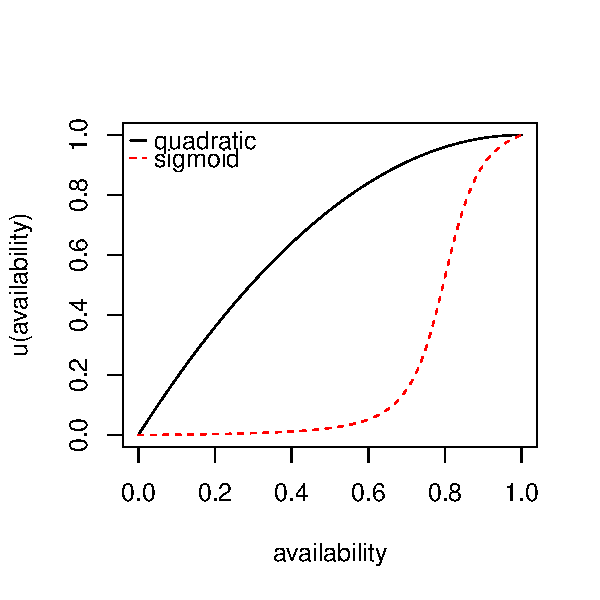
\includegraphics{fig-optim2/quad-sig.pdf}
  \caption{Comparison of the (risk averse) quadratic utility function, and the sigmoidal utility function.}
  \label{Fig:quad-sig}
\end{figure}

The ``$1$ minus'' indicates a quadratic utility function but this takes into account that the smaller values of $c_2$, $c_3$ are better, this also expresses risk aversion. Conversely, large values of $c_1$ are better. The notation $c_1^{(j)}$ means the $j$th time point in the availability time series (which has approximately uniform intervals) and $c_{3,j}$ is the $j$th critical percentage. This utility function represents the idea that we would want to maximise availability whilst minimising overheads. We take the weights here to be $(0.8,0.1,0.1)$.




Now, the consequences are (possibly stochastic) functions of the decision variables so from hereon in we write $u$ as a function of $\bx$.

\section{Optimisation Strategy}

The problem now is to find the global maximum of $U(\bx)$ and the corresponding maximiser. Since $u(\bx)$ is expensive and stochastic we will use Bayesian optimisation to find the optimal decision. The three choices of warehouse lead to the number of spares lying on a different simplex-like space (and cover different ranges) so we will use three independent Gaussian processes to model the utility function conditional on the choice of warehouse. Denote the utility function, conditional on choice of warehouse by $u(\bx|w)$. Therefore we will proceed by maximising each $U(\bx|w)$ w.r.t. $\bx$. Global maximisation over the entire decision space can be achieved by maximising $U(\hat{\bx}_w|w)$ w.r.t. $w$, where $\hat{\bx}_w$ is the decision maximising $U(\bx|w)$.

Now, we could proceed by simply maximising $U(\bx|w)$ using standard Bayesian optimisation acquisition functions such as EI or PI \citep{Shahriari2015}. However, since the utility function outputs values on $[0,1]$ the standard Gaussian assumptions for the expected value likely will be violated. This can be alleviated with moderate to large amount of replication depending on how severe the deviations from Normality are.
%The machine learning community frequently have little concern about knowledge of the output space and will happily maximise, e.g. probabilities or proportions using acquisition function which don't take into account the structure of the output space \citep{Moss2020} - the lack of concern is likely due to Bayesian optimisation working quite well despite these constraints.
In the statistical literature when using GPs to model quantities constrained to the unit interval (or known finite interval), the unwritten rule is to model the a transformed version of this quantity by a GP. For instance, \citet{Henderson09, Boys2018,Baker2020c} all model the logit output to allow the quantity of interest to be unconstrained, which is far more appropriate for GP based models. The advantage of the logit based approach is that all predictions and interval estimates are in some sense valid (i.e. will not spill outside of $(0,1)$). The transformation is usually quite successful in giving us an (approximately) additive noise structure. Further, in the appendix we argue that the logit transform provides the appropriate transformation for random variables which are either Beta distributed, or whose logit is Normally distributed. %A major disadvantage of this approach is that maximising $\E \{ \logit u(\bx) \} $ will not give the same answer as maximising $U(\bx)$ unless $u(\bx)$ is a deterministic function of $\bx$.

Our approach will be to utilise the logit transformation and use an acquisition function that has knowledge of the transformation. In the spirit of \citet{Oakley2009} we construct the emulator for $\logit U(\bx)$ rather than for any expensive computer models. There are a few reasons for this. First, it gives us easier access to $\E \{ U(\bx) \}$ (Oakley achieves direct access). When combining multiple model outputs from the same model, or an ensemble of models this avoids emulating many, possibly correlated, outputs. For instance, Athena outputs a time series which will exhibit strong serial correlation. Although emulation of time series outputs (\textit{dynamic codes}) is well studied \citep{Conti2009, Conti2010, oyebamiji2017}, emulation of the utility function provides automatic dimension reduction to a scalar response.

We use an acquisition function based on expected improvement (EI) due to it being well understood and relative simplicity. In fact, we simply propose to use EI under a more appropriate statistical model.
If $f(\cdot)$ is modelled by a GP then
\begin{align}
  \EI (\bx) &= \E_{f(\cdot)} \max \{0,  f(\bx) - \hat{y} \}\\
    &= \left( \mu(\bx) - \hat{y} \right) \Phi \left[ \frac{\mu(\bx) - \hat{y}}{\sigma(\bx)} \right]  + \sigma(\bx) \phi \left[ \frac{\mu(\bx) - \hat{y}}{\sigma(\bx)}\right]
\end{align}
where $\hat{y}$ is the largest known simulator value (or largest expected simulator value in the stochastic case). Traditionally, $f(\cdot)$ is modelled by a GP.

  We suggest modelling the logit utility function by a GP. We use a constant nugget effect, constant mean function and squared exponential covariance function:

\begin{equation}
  \logit u(\cdot) \sim \mathcal{GP} \{ \beta, C(\cdot, \cdot) \}
\end{equation}
with
\begin{equation}
  C(\bx, \bx') = \sigma^2 \exp \{ -(\bx - \bx)^T D^{-1} (\bx - \bx') \} + \lambda^2 \delta_{\bx , \bx'}
\end{equation}

where $\sigma$ is a scale parameter, $D$ is a (diagonal) matrix of lengthscale parameters, $\lambda$ is the noise standard deviation and $\delta_{\bx, \bx'}$ is Kronecker's delta. Although $\lambda$ is a catch all for `noise' it serves two purposes here. Firstly, to capture genuine stochasticity in simulations, but also to account for the epistemic uncertainty about model parameters which have been assigned prior distributions in Athena. Having observed data, $\mathcal{D}_n = \{ (y_1, \ldots, y_n), (\bx_1, \ldots, \bx_n)\}$ the `time $n$' posterior distribution (that being, the posterior having observed $n$ simulator runs) of $\logit u(\bx)$ is Gaussian with mean $m(\bx)$ and variance $s^2(\bx)$. Prediction intervals can be found by adding $\lambda^2$ to $s^2(\bx)$. After running the optimisation scheme, we find the optimal decision by
\begin{equation}
  \hat{\bx}^{*} = \argmax_{\bx \in X} \E \{ U(\bx) \}
\end{equation}
where $X$ is the set of decisions which have been queried. Expectation is taken with respect to the posterior distribution of $U(\cdot)$.
Now under this approach, with maximisation in mind and the current largest expected value being $\hat{y}$,  the expected improvement is

\begin{equation}
  \EI(\bx) = \int_{\hat{y}}^1 \frac{\exp \left\{  -\frac{1}{2}\left( \frac{\logit(y) - m(\bx)}{s(\bx)}\right) ^2 \right\}}{s(\bx)\sqrt{2 \pi} (1 - y)} - \hat{y} \diff y. \label{Eq:EI-logitn}
\end{equation}

However, the form in \Cref{Eq:EI-logitn} can be numerically unstable due to the division by $1-y$. It is much more numerically stable reprase $\EI(\bx)$ as $\E_Z \{ \max [  \expit(m(\bx) + s(\bx)) - \hat{y}, 0 ] \} $ where $Z \sim N(0,1)$. This leads to the following form of the integral
\begin{equation}
  \EI(\bx) = \int_{z_{\hat{y}}}^{\infty} \expit\{m(\bx) + s(\bx)z\} \phi(z) \diff z \label{Eq:EI-logitn2}
\end{equation}
 where $z_{\hat{y}} = (\logit (\hat{y} )- m(\bx))/s(\bx)$. The form in \Cref{Eq:EI-logitn2} which avoids division by small numbers unless $s(\bx$) is tiny. Howeber, this is present in both forms.
If we want to minimise the function (e.g. minimise a loss function) we could maximise $1-f(\bx)$. Unfortunately, the integral term is intractable but can be easily computed using numerical methods. We use \verb|integrate| from \verb|R| (on the form in \Cref{Eq:EI-logitn2}) which is an adaptive quadrature method for integration. This is usually numerically stable but can fail when the logit-Normal density is almost zero everywhere except for a spike close to $1$ (e.g. if both $m(\bx)$ and $s(\bx)$ are large). When the integral fails, we can Riemann sum approximation. It is generally less accurate than the adaptive quadrature approach so is only used as a last resort.

BayesOpt using transformed Normal densities has been considered other scenarios. \citet{Nguyen2020} consider a $\chi ^2$ process when the maximum value (but not the maximiser) is known, in our case we have some upper (and lower) limits, $(a,b)$ which we know the maximiser sit between: $a < U(\bx^{*}) < b$.
\subsection{Maximising the Acquisition Function}

To choose the next point at which to evaluate the utility function we need to maximise the acquisition function. That is

\begin{equation}
  \bx_{n+1} = \argmax_{\bx \in \mathcal{X}_w} \EI(\bx).
\end{equation}

Now since the number of spare components sits on an integer simplex maximisation isn't straightforward. For now, we implement a slight fudge. We treat $\EI(\bx)$ as if it is valid for the space $\mathcal{X}_{w}' = \mathcal{S}^{(w)}_9 \times [0.05,0.95]^9$ where $S^{(w)}_9$ is a continuous-valued $9D$ simplex rescaled to give the correct range of spare parts. We then find the global maximum of $\EI(\bx)$ on $\mathcal{X}_{w}'$ via \verb|L-BFGS-B| in \verb|optim|. We then round to a nearby element of $\mathcal{X}_s^{(w)}$ by calculating the EI at all `corners' around the maximiser of the relaxed problem. In essence, we relax the discrete nature of the optimisation problem and then round to the best solution in a region close to the relaxed maximiser. This could be made more `exact' (but slower) by using an optimisation approach such as simulated annealing to maximise the acquisition function; this would only consider valid solutions to the problem.


\section{Maximisation via EI}

Here we apply the discussed BayesOpt methodology to the decision problem. Consider the three warehouse set up as before and a computational budget of $250$ runs for each warehouse ($750$ runs in total, distributed equally). The first $40$ runs ($40 \approx 2 \times \text{input space dimension}$) were chosen via random sampling to infer inital GP hyperparameters. We used a random designs rather than more complex designs schemes such as maximin or Latin hypercubes because random is trivial to implement in the simplex case. There is also empirical evidence that learning GP hyperparameters is more effective under a random design than the space-filling alternatives \citep{Zhang2019}. The remaining runs for each warehouse are then chosen sequentially via the Expected Improvement strategy explained above.

\begin{figure}
  \centering
  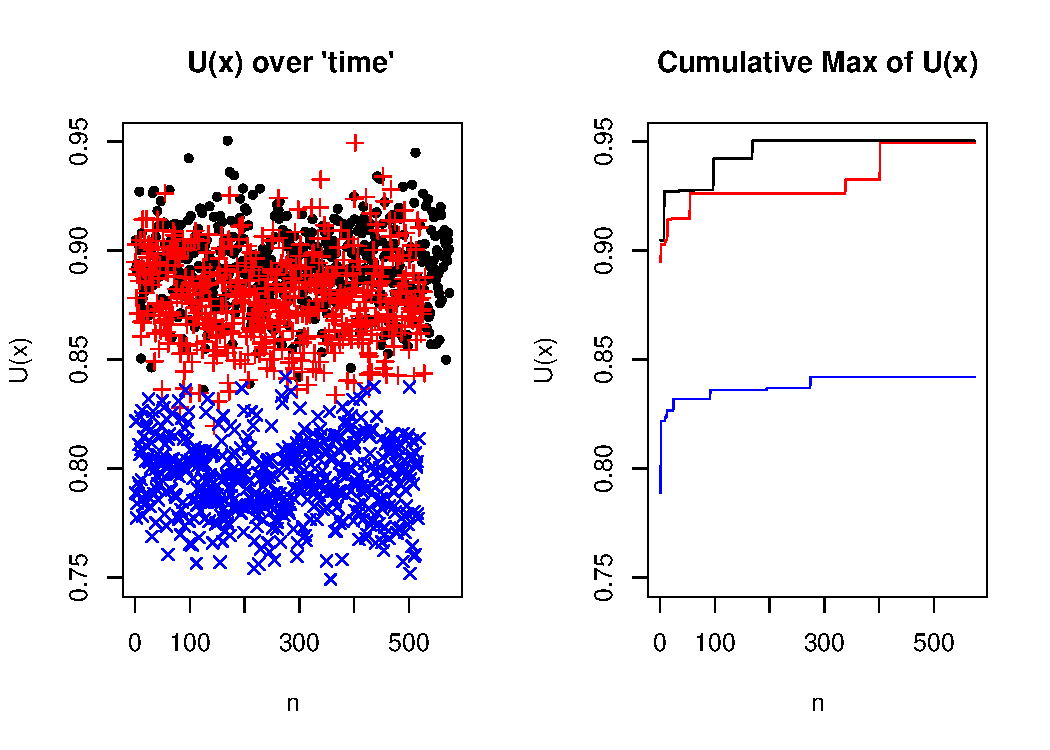
\includegraphics[width=\textwidth]{fig-optim2/trace-EI2.pdf}
  \caption{Left hand plot shows the smoothed value of $U(\bx_n)$ (posterior mean), separated by warehouse. Right hand plot shows the cumulative maximum, also separated by warehouse. Black dots/line corresponds to warehouse $1$, red $+$/line to warehouse $2$ and blue $\times$/line to warehouse $3$.}
  \label{Fig:EI-trace}
\end{figure}


As mentioned, the global optimisation was split into three sub-optimisations which were run in parallel. This is possible because we treat the model runs as independent of each other, if they corresponds to a different choice of warehouse. We argue that this is the most appropriate course of action because the input spaces for different warehouses are disjoint. %As illustrated in \Cref{Fig:Simplices}.
 This prevents spurious correlations being induced across warehouses but also reduces the size of covariance matrices so acquisition calculations are $\mathcal{O}(n^2 )$ rather than $\mathcal{O}((3n)^2)$, given the GP precision matrix (if the precision matrix is unknown but the covariance matrix is known, the powers go from squares to cubes). Further, because the three implementations are done independently, the three sub-optimisations can be trivially parallelised.

%\begin{figure}
%  \centering
%  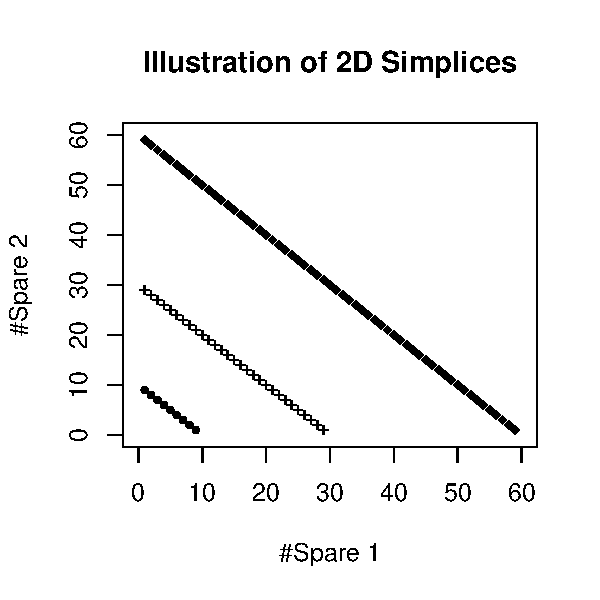
\includegraphics{fig/simplices.pdf}
%  \caption{Simplices for a version of our problem with just $2$ types of spares. Dots correspond to a warehouse of size $10$, plus symbols of size $30$ and the diamonds as size $60$.}
%  \label{Fig:Simplices}
%\end{figure}
We choose to terminate the optimisation when either $24$ hours of computation time had elapsed or we had made $1000$ queries to Athena (which ever occured first). Here, we define a single query as $20$ replications of Athena at the same input vector. The first $40$ runs were chosen at random to train the GP and the remaining runs were chosen sequentially.In all three cases, the time limit was met before the limits on the number of runs. We obtained $574$, $529$ and $518$ queries for warehouses $1$, $2$ and $3$ respectively.

\section{Maximisation via Upper Quantile}

We can also try maximisation via the UCB approach. Again, we alter the UCB acquisition function to take into account the fact that $U(\bx) \in (0,1)$. In this case the UCB really becomes an upper quantile (UQ) heuristic. Since the logit-Normal is obtained by an increasing, one-to-one transformation of the Normal distribution, the $q^{th}$ quantile of the logit-Normal distribution is just the expit of the corresponding quantile of the Normal distribution.  Therefore we have
\begin{align}
  \alpha_{UQ}(\bx \mid \nu_n ) = \expit\{ \mu_n(\bx) + \nu_n \sigma_n(\bx) \}
\end{align}
where $\nu_n$ are a sequence of (positive) tuning parameters. We express this acquisition function in a similar way to the UCB heuristic, but $\nu_n$ could easily be expressed as a quantile by means of the Normal CDsame as maxF. Because $\expit(\cdot)$ is a increasing and monotonic function, maximising $\alpha_{UQ}(\bx \mid \nu_n)$ is the same as maximising $\alpha_{UCB}(\bx \mid \nu_n) = \mu_n(\bx) + \nu_n \sigma_n(\bx)$ so we will do precisely this. That is
\begin{equation}
  \bx_{n+1} = \argmax_{x \in \mathcal{X}_w} \mu_n(\bx) + \nu_n \sigma_n(\bx).
\end{equation}
 We can use similar tricks to maximise $\alpha_{UQ}$ as the $\EI$ heuristic, but in this case the acquisition function is analytically tractable. We used the same stopping rules in this optimsation, however in this case we reached the $1000$ point limit in $17.5$ hours, $18$ hours and $14.25$ hours for warehouses $1$, $2$ and $3$. Again, we use L-BFGS-B for maximisation of the acquisition function with the gradient supplied. In this case we observed utilities are increasing approximately linearly with $n$ in all cases.


\begin{figure}
  \centering
  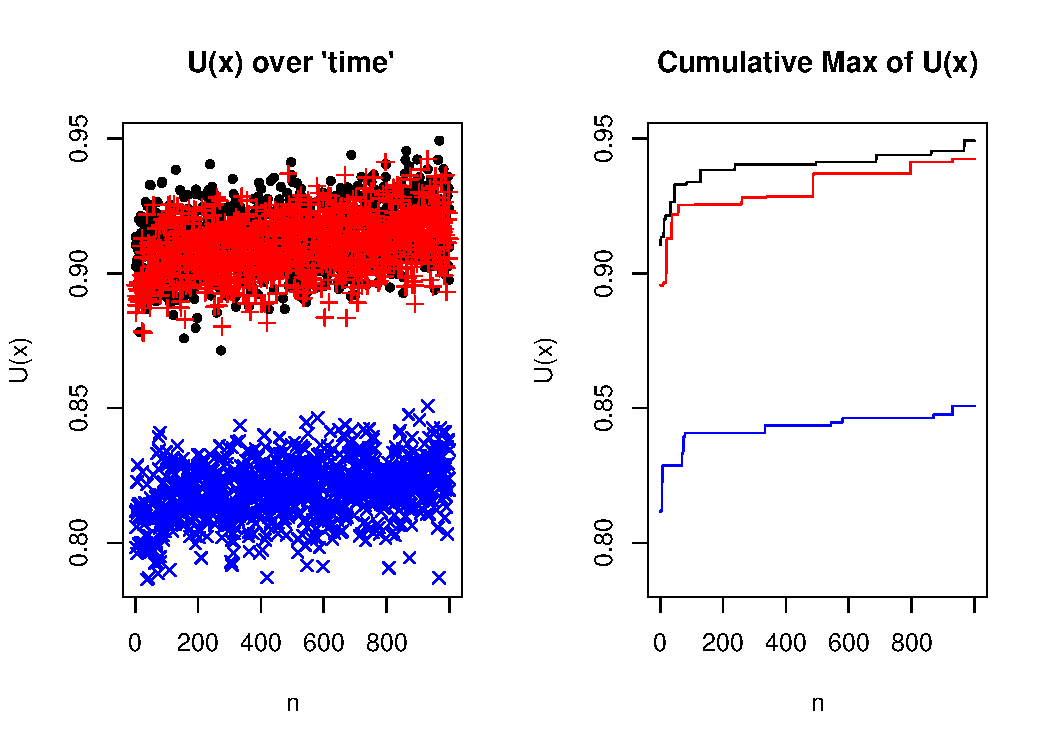
\includegraphics[width=\textwidth]{fig-optim2/ucb-trace2.pdf}
  \caption{Left hand plot shows the smoothed value of $U(\bx_n)$ (posterior mean), separated by warehouse. Right hand plot shows the cumulative maximum, also separated by warehouse. Black dots/line corresponds to warehouse $1$, red $+$/line to warehouse $2$ and blue $\times$/line to warehouse $3$.}
  \label{Fig:ucb-trace}
\end{figure}


The results of maximisation via UQ broadly agree with the EI maximisation. That is, the smallest warehouse is most preferred and the largest warehouse is least preferred. The maximum of each warehouse is approximately the same in each case.

The time $n$ optimal decision under each heuristic has the following expected utility $\E \{U(\bx^{*}_{UQ})\} = 0.949$ and $\E \{U(\bx^{*}_{EI})\} = 0.950$, both to $3$ decimal places. The optimal decisions are for the smallest warehouse. The values of the remaining parameters are given in \Cref{Tab:opt-dec}.
\begin{table}
  \centering
  \begin{tabular}{lrrrrrrrrr}
    \toprule
    $i$ & 1 &2& 3& 4& 5& 6 &7 &8 &9 \\
    & 10& 11& 12& 13& 14& 15& 16& 17& 18 \\\cmidrule{1-10}
    $\bx_{UQ}$ & 1 & 3 & 1  & 39  & 1 & 1  & 1  & 1  & 2 \\
     & 11.43 & 48.73 & 39.14 & 17.99 & 63.81 & 7.94 & 24.29 & 27.68 & 7.99  \\\cmidrule{1-10}
    $\bx_{EI}$ & 39 & 1 & 1 & 1 & 1 & 2 & 1 & 2 & 3 \\
      &  5.45 & 2.13 & 17.86 & 17.48 & 7.95 & 7.61 & 19.05 & 98.01 & 22.08  \\
    \bottomrule
  \end{tabular}
  \caption{Optimal decision under each of the considered BayesOpts heuristics. Top row represents $x_1$ -- $x_9$, bottom row represents $x_{10}$ -- $x_{18}$. In each case, the estimated global maxiumum is attributed to warehouse $1$.}
  \label{Tab:opt-dec}
\end{table}

\section{Post-Hoc Analysis}

Although both optimisation runs suggest that the smallest warehouse almost always leads to the best decision, the result is very tight. There are at least two sources of uncertainty that we ought to consider prior to commiting to the decision:
\begin{itemize}
  \item[(a)] Athena is stochastic thus expected utilities are obfuscated by noise
  \item[(b)] the computational expense of simulations means the decision space cannot be fully explored.
\end{itemize}
There are also other uncertainties, for example model discrepancy. For now we take model discrepancy to be $0$ (with $0$ variance), this is unrealistic but could be added into the analysis at a later date with the help of expert judgement.

 The choice of warehouse is a permanent decision. Once the warehouse is up an running, it would be highly impractical or perhaps impossible to move to another unit because, for instance, the warehouses within an appropriate locality are now being used by another business. However, if the wind farm operator realised the DM's prior over failure rates was poorly calibrated with reality, it would be relatively easy to adjust how frequently spare parts are ordered in and adapt the allocation of spares in near-real time.

To quantify our confidence in the choice of warehouse we propose to use history matching (HM) inspired idea. We will investigate which decisions cannot be ruled out as inconsistent with the `current' optimal decision. We use the word `current' here since learning more about the utility function, by running more simulations, could change the optimal decision. There is also the fact that a DM is encouraged to change their utility function and priors as soon as they realise the utility function and priors are not a faithful representation of their preferences and beliefs.

Our approach is to use an implausibility measure to rule out decisions which are, given all relevant uncertainties, sufficiently different (and smaller in expected utility) than the time $n$ optimal decision. HM is an approach to calibrating computer models to data \citep{Vernon14, andrianakis2017a} but has inspired useful statistical methods outside of calibration. For instance, \citet{Baker2020c} use HM techniques for level set estimation and \citet{Wang2018} use HM techniques to investigate prior predictive distributions for Bayesian analysis. A HM based optimisation procedure was introduced by \citet{Lawson2016}. They used a HM approach to iteratively refocus emulators towards the function's maximum value. We propose to use a HM inspired technique to investigate how robust the choice of warehouse is. The purpose is to inspire confidence in the decision maker when the choice of warehouse is clear. Conversely, the approach will also make the DM aware that their decision is potentially sub-optimal, given key uncertainties.

We propose using the following implausibility measure

\begin{align}
  \mathcal{I}(\bx) &= \frac{ \E \left\{ U(\hat{\bx}) - U(\bx)\right\}}{\var \left\{ U(\hat{\bx}) - U(\bx)\right\}^{1/2} }\\
  &=\frac{\E \left\{ U(\hat{\bx}) \}  - \E \{U(\bx)\right\}}{ \left\{ \var(U(\hat{\bx})) + \var(U(\bx)) - 2\cov(U(\bx), U(\hat{\bx})) \right\}^{1/2} }.
\end{align}
Here, expectations, variances and covariances are with respect to the posterior distribution of the relevant GPs. We also abuse notation slightly here and allow $\bx$ to also encode the choice of warehouse and $\hat{\bx}$ denotes the current optimal decision (including choice of warehouse). Note that, if the warehouses are different the covariance term vanishes because the emulators were constructed independently of each other. If the warehouse for $\bx$ and $\hat{\bx}$ is the same, or we built a joint statistical model for the warehouses then the covariance in general will be non-zero.

The implausibility needs to be coupled with a cut-off to `rule out' decisions. We will use $\mathcal{I}(\bx) = 3$ as the cut off. The choice of $3$ makes a good default and is justified by Pukelsheim's $3\sigma$ rule \citep{Pukelsheim1994}. The $3\sigma$ rule relies on a unimodal distribution; the logit-Normal distribution can be bimodal. The mode satisfies $\logit (x) = \sigma^2 (2x - 1) + \mu$. We can check the number of solutions to this equation for every instance, but realistically, the number of solutions will be $1$ when the uncertainty is not too large. This can be achieved by reducing uncertainty though an appropriate number of model runs, but also MAP/Bayesian estimation of GP hyperparameters allows us to somewhat control multi-modality by including useful prior information. HM typically incorporates model discrepancy but we have ignored that notion here - it could however be included to account for discrepancy in Athena induced by modelling simplifications, discretisation and imprecision in the DM's utility function. Note that in the standard HM framework, the measure would usually be non-negative. Here we allow for negative implausibility to indicate that the expected utility of a decision which has yet to be investigated could be \textit{larger} than $U(\hat{\bx})$.

First we investigate the points are which the model has already been run, these decisions will typically have the least uncertainty about them. For this part we will just run the analysis on the results from the $UQ$ acquisition function. Although the $\EI$ acquisition gave us a (marginally) better solution, this is only an estimate of the solution. The $UQ$ emulators contain approximately double the amount of data from which to make predictions thus might be considered more trustworthy.

 From \Cref{Fig:hm-ucb} there is little overlap so we should expect the implausibility to be large and positive.
\begin{figure}
  \centering
  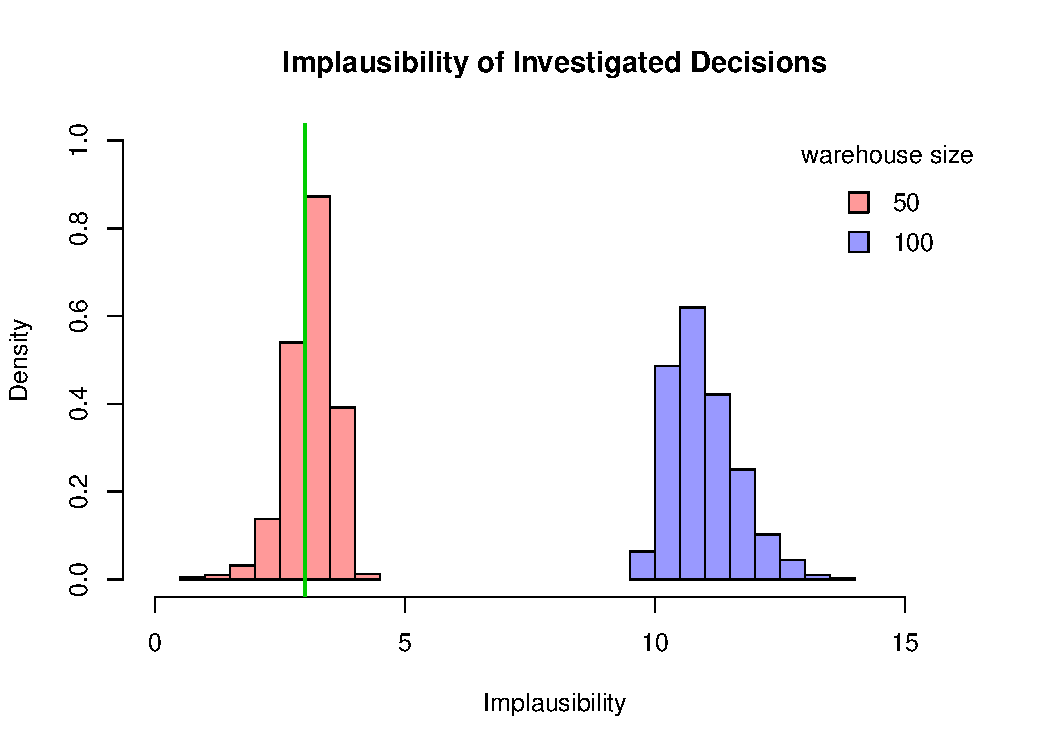
\includegraphics[width=0.8\textwidth]{fig-optim2/hm-ucb2.pdf}
  \caption{Implausibility for the already considered decisions from the warehouses of sized $50$ and $100$, here the data corresponds to that obtained under the UQ acquisition function. Vertical green line is at the cut off $\mathcal{I}(\bx)=3$. }
  \label{Fig:hm-ucb}
\end{figure}

We suspected that the larger warehouses would be appreciably worse decisions and this is verified by \Cref{Fig:hm-ucb}; the smallest implausibility is around $0.805$ which is a lot less than the cut-off; we cannot `rule out' warehouse $2$ as a sensible decision. However, we should check that we cannot also rule out warehouse $3$ by considering the implausibility of inputs which have not yet been run. This can be achieved by minimising the implausibility, but we have an alternative here which is computationally very simple and efficient. We just need to show that the time $n$ best decision is much larger that $0.9$ which is the maximum possible utility for warehouse $3$. Note that for time $n$ optimal decision is characterised by $\logit U(\hat{\bx}_n) \sim \mathcal{N}(2.94, 0.0180)$. From this, we can calculate $(\E \{ U( \hat{\bx}_n ) \} - 0.9 )/ \sqrt{ \var \{ U( \hat{\bx}_n) \} ) } = 7.62 > 3$ thus warehouse $3$ can be ruled out without any intensive computations.





\section{Conclusion}

We have found (approximately) the optimal decision in a resource allocation problem concerning large offshore wind farms. This was achieved with Bayesian optimisation with an EI acquisition function under the assumption of either a logit-Normal or Beta distributed simulator output.

We then applied a HM inspired approach to investigate how robust the choice of warehouse is to deviation in the fine tuning of the decision. We showed, given all relevant uncertainties, that the $50$ capacity warehouse was certaainly preferable to the $100$ capacity warehouse. However, the $75$ capacity warehouse was not ruled out yet. This means that if further resources (computational, financial) are available, they should be put into investigating the two smaller warehouses. If we were able to rule out both of the larger warehouses completely, we could then pour all remaining resources into the smallest (best) warehouse to fine tune that particular warehouse as much as possible.

\end{chapter}
